\chapter{Hexahedral Quality Metrics\label{s:hex}}

All the metrics in this section are defined on a hexahedral element
as shown in Figure~\ref{f:hex}.
Unless noted otherwise, hexahedra are assumed to have planar faces.

\begin{figure}[bhp]
  \centering
  \includegraphics[width=2.5in]{hex}
  \caption{A prototypical hexahedral finite element.%
                                                                  \label{f:hex}}
\end{figure}

We index the edges as follows.
Note that order of the edges does \textbf{not} match \vtk.
\begin{equation*}
\begin{array}{lclcl}
  \vec L_0    &=& \vec P_1 - \vec P_0\\
  \vec L_1    &=& \vec P_2 - \vec P_1\\
  \vec L_2    &=& \vec P_3 - \vec P_2\\
  \vec L_3    &=& \vec P_3 - \vec P_0
\end{array}\rule{2em}{0pt}
\begin{array}{lclcl}
  \vec L_4    &=& \vec P_4 - \vec P_0\\
  \vec L_5    &=& \vec P_5 - \vec P_1\\
  \vec L_6    &=& \vec P_6 - \vec P_2\\
  \vec L_7    &=& \vec P_7 - \vec P_3
\end{array}\rule{2em}{0pt}
\begin{array}{lclcl}
  \vec L_8    &=& \vec P_5 - \vec P_4\\
  \vec L_9    &=& \vec P_6 - \vec P_5\\
  \vec L_{10} &=& \vec P_7 - \vec P_6\\
  \vec L_{11} &=& \vec P_7 - \vec P_4
\end{array}
\end{equation*}

The tetrahedron edge lengths are denoted as follows:
\[
L_0 = \normvec{L_0}\quad
\dots\quad
L_{11} = \normvec{L_{11}}
\]
and the largest and smallest edge lenghts are, respectively,
\begin{equation*}
\begin{array}{lcl}
  L_{\min} &=& \min\left\{L_0, \dots, L_{11} \right\}\\
  L_{\max} &=& \max\left\{L_0, \dots, L_{11} \right\}.
\end{array}
\end{equation*}

Hexahedra have four diagonal vectors:
\begin{equation*}
\begin{array}{lcl}
\vec D_0 &=& \vec P_6 - \vec P_0\\
\vec D_1 &=& \vec P_7 - \vec P_1
\end{array}\rule{10em}{0pt}
\begin{array}{lcl}
\vec D_2 &=& \vec P_4 - \vec P_2\\
\vec D_3 &=& \vec P_5 - \vec P_3
\end{array}
\end{equation*}

\begin{equation*}
\begin{array}{lcl}
  D_{\min} &=& \min\left\{\normvec{D_0},\normvec{D_1},\normvec{D_2},\normvec{D_3} \right\}\\
  D_{\max} &=& \max\left\{\normvec{D_0},\normvec{D_1},\normvec{D_2},\normvec{D_3} \right\}
\end{array}
\end{equation*}

The principal axes are
\begin{equation*}
\begin{array}{lcl}
  \vec X_1 &=&
    \left(\vec P_1-\vec P_0\right) + \left(\vec P_2-\vec P_3\right) +
    \left(\vec P_5-\vec P_4\right) + \left(\vec P_6-\vec P_7\right)\\
  \vec X_2 &=&
    \left(\vec P_3-\vec P_0\right) + \left(\vec P_2-\vec P_1\right) +
    \left(\vec P_7-\vec P_4\right) + \left(\vec P_6-\vec P_5\right)\\
  \vec X_3 &=&
    \left(\vec P_4-\vec P_0\right) + \left(\vec P_5-\vec P_1\right) +
    \left(\vec P_6-\vec P_2\right) + \left(\vec P_7-\vec P_3\right)\\
\end{array}
\end{equation*}

The cross derivatives are then
\begin{equation*}
\begin{array}{lclcl}
  \vec X_{12} &=& \vec X_{21} &=&
    \left(\vec P_2-\vec P_3\right) - \left(\vec P_1-\vec P_0\right) +
    \left(\vec P_6-\vec P_7\right) - \left(\vec P_5-\vec P_4\right) \\
  \vec X_{13} &=& \vec X_{31} &=&
    \left(\vec P_5-\vec P_1\right) - \left(\vec P_4-\vec P_0\right) +
    \left(\vec P_6-\vec P_2\right) - \left(\vec P_7-\vec P_3\right) \\
  \vec X_{23} &=& \vec X_{32} &=&
    \left(\vec P_7-\vec P_4\right) - \left(\vec P_3-\vec P_0\right) +
    \left(\vec P_6-\vec P_5\right) - \left(\vec P_2-\vec P_1\right) \\
\end{array}
\end{equation*}

We can define a series of $3\times 3$ Jacobian matrices on a given hexahedron using
the edge vectors $\vec L_i$ to form columns of each matrix:
\begin{equation*}
\begin{array}{lrrcrcrl}
A_0 &= (&  \vec L_0   &,&  \vec L_3   &,&  \vec L_4 &)\\
A_1 &= (&  \vec L_1   &,& -\vec L_0   &,&  \vec L_5 &)\\
A_2 &= (&  \vec L_2   &,& -\vec L_1   &,&  \vec L_6 &)\\
A_3 &= (& -\vec L_3   &,& -\vec L_2   &,&  \vec L_7 &)\\
A_4 &= (&  \vec L_{11}&,&  \vec L_8   &,& -\vec L_4 &)\\
A_5 &= (& -\vec L_8   &,&  \vec L_9   &,& -\vec L_5 &)\\
A_6 &= (& -\vec L_9   &,&  \vec L_{10}&,& -\vec L_6 &)\\
A_7 &= (& -\vec L_{10}&,& -\vec L_{11}&,& -\vec L_7 &)\\
A_8 &= (&  \vec X_1   &,&  \vec X_2   &,&  \vec X_3 &)
\end{array}
\end{equation*}
These matrices will be useful in calculating the volume and condition number of a hexahedron.
Some operations we will need to perform on these matrices can be reduced to simple vector operations.
Since this is how we define the matrices, these forms of the operations serve as efficient implementations.

Let $A$ be one of these $3 \times 3$ matrix defined by the
column vectors $\vec v_1, \vec v_2, \vec v_3,$ i.e., $A = [\vec v_1, \vec v_2, \vec v_3]$. 
Then, 
\[
|A|^2 = \normvec{ v_1}^2 + \normvec{ v_2}^2 + \normvec{ v_3}^2 
\]
and
\[
|\mathrm{adj}(A)|^2 = \normvec{ v_1 \times \vec v_2}^2 + 
             \normvec{ v_2 \times \vec v_3}^2 +
             \normvec{ v_3 \times \vec v_1}^2 .
\]
We then define $\alpha$ to be the determinant of $A$
\[
\alpha = \det(A) = \vec v_1 \cdot (\vec v_2 \times \vec v_3 )
\]
and we denote the determinant of a specific one of the $A_i$ as
\[
\alpha_i = \det(A_i)
\]
where $i\in\{0,1,\ldots,8\}$.
Finally, we define normalized versions of the Jacobian matrices
\[
  \hat A = \left(
    \frac{\vec v_1}{\normvec{ v_1}}\;,
    \frac{\vec v_2}{\normvec{ v_2}}\;,
    \frac{\vec v_3}{\normvec{ v_3}}
  \right)
\]
and their normalized determinants
\[
  \hat\alpha_u = \det\left(\hat A_i\right).
\]

% -------------------Metric Table-------------------
\newcommand{\hexmetrictable}[8]{%
  \begin{center}
  \begin{tabular}{ll}
    \multicolumn{2}{r}{\textbf{\sffamily\Large hexahedral #1}}\\\hline
    Dimension:             & #2\\ 
    Acceptable Range:      & #3\\ 
    Normal Range:          & #4\\ 
    Full Range:            & #5\\ 
    $q$ for unit cube:     & #6\\
    Reference:             & #7\\
    \verd\ function:       & \texttt{#8}\\ \hline
  \end{tabular} 
  \end{center}
}

\newpage %---------------------------Diagonal---------------------------
\section{Diagonal}

This metric is the ratio of the minimum diagonal length to the maximum diagonal length:
\[
q = \frac{D_{\min}}{ D_{\max}}.
\]
Note that if $D_{\max} < DBL\_MIN$, we set $q = DBL\_MAX$.

\hexmetrictable{diagonal}%
{$1$}%                                        Dimension
{$[0.65,1]$}%                                 Acceptable range
{$[0,1]$}%                                    Normal range
{$[1,DBL\_MAX]$}%                             Full range
{$1$}%                                        Cube
{--}%                                         Citation
{v\_hex\_diagonal}%                           Verdict function name

\newpage %---------------------------Dimension---------------------------
\section{Dimension} 

This metric was specifically designed in the context of
Sandia's \textsf{Pronto} code, for stable time step calculation. It is
defined as follows:
\[
q = \frac{V}{2\nabla{V}}
\]
\hexmetrictable{dimension}%
{$L^1$}%                                      Dimension
{application-dependent}%                      Acceptable range
{$[0,DBL\_MAX]$}%                             Normal range
{$[0,DBL\_MAX]$}%                             Full range
{$1$}%                                        Cube
{Adapted from \cite{tf:89}}%                  Citation
{v\_hex\_dimension}%                          Verdict function name

\newpage %---------------------------Distortion---------------------------
\section{Distortion} 

Given a set of Gauss points $G=\{g_k\}$ for a hexahedron, let
\[
|J| = \min_{g_k}\left\{\det\left(J_{g_k}\right)\right\}
\]
be the minimum determinant of the Jacobian when evaluated at each Gauss point $g_k$.
Then the distortion is
\[
q = \frac{|J| V_m}{V}  
\]
where $V_m = 8$ is the volume of a ``master'' hexahedron defined by the vertices
\[
\begin{array}{lcrcrcrl}
  \vec P_0 &= (&-1&,&-1&,& -1&)\\
  \vec P_1 &= (& 1&,&-1&,& -1&)\\
  \vec P_2 &= (& 1&,& 1&,& -1&)\\
  \vec P_3 &= (&-1&,& 1&,& -1&)
\end{array}\rule{5em}{0pt}
\begin{array}{lcrcrcrl}
  \vec P_4 &= (&-1&,&-1&,&  1&)\\
  \vec P_5 &= (& 1&,&-1&,&  1&)\\
  \vec P_6 &= (& 1&,& 1&,&  1&)\\
  \vec P_7 &= (&-1&,& 1&,&  1&)
\end{array}
\]
and $V$ is the volume of the hexahedron being evaluated.
See \S\ref{s:hex-volume} for details on computing the hex volume $V$.

\hexmetrictable{distortion}%
{$L^3$}%                                      Dimension
{$[0.5,1]$}%                                  Acceptable range
{$[0,1]$}%                                    Normal range
{$[-DBL\_MAX,DBL\_MAX]$}%                     Full range
{$1$}%                                        Cube
{Adapted from \cite{ideas:xx}}%               Citation
{v\_hex\_distortion}%                         Verdict function name

\newpage %---------------------------Shape-----------------------------
\section{Edge Ratio\label{s:hex-edge-ratio}}

The edge ratio quality metric is the ratio of the longest to
shortest edge of a hexahedron:
\[
q = \frac{L_{\max}}{L_{\min}}.
\]

\hexmetrictable{edge ratio}%
{$1$}%                                        Dimension
{--}%                                         Acceptable range
{$[1,DBL\_MAX]$}%                             Normal range
{$[1,DBL\_MAX]$}%                             Full range
{$1$}%                                        Cube
{--}%                                         Citation
{v\_hex\_edge\_ratio}%                        Verdict function name

\newpage %---------------------------Jacobian---------------------------
\section{Jacobian}

This is the minimum determinant of the Jacobian matrix evaluated at each corner and the center of the element:
\[
q = \min\left\{\left\{\alpha_i\right\}_{i=0}^7, \frac{\alpha_8}{64} \right\}.
\]
This can also be interpreted as the minimum pointwise volume of local map
at the 8 corners and the center of the hexahedron.

\hexmetrictable{Jacobian}%
{$L^3$}%                                      Dimension
{$[0,DBL\_MAX]$}%                             Acceptable range
{$[0,DBL\_MAX]$}%                             Normal range
{$[-DBL\_MAX,DBL\_MAX]$}%                     Full range
{$1$}%                                        Cube
{\cite{knu:00}}%                              Citation
{v\_hex\_jacobian}%                           Verdict function name

\newpage %---------------------------Maximum Edge Ratio---------------------------
\section{Maximum Edge Ratio}

Given principal axes with lengths $L_f$ and $L_g$,
the aspect ratio is defined as the largest ratio of those lengths
\[
   A_{fg} = \max\left\{ \frac{L_f}{L_g}, \frac{L_g}{L_f} \right\}.
\]
Since a hexahedron has 3 principal axes, we take the largest of all pairwise combinations of axes.
\[
  q  = \max\left\{
    A_{\normvec{ X_1 }\normvec{ X_2 }},
    A_{\normvec{ X_1 }\normvec{ X_3 }},
    A_{\normvec{ X_2 }\normvec{ X_3 }}
  \right\}
\]

Note that if $\normvec{X_1}$ or $\normvec{X_2}$ or $\normvec{X_3} < DBL\_MIN$, we set $q = DBL\_MAX$.

\hexmetrictable{maximum edge ratio}%
{$1$}%                                      Dimension
{$[1,1.3]$}%                                Acceptable range
{$[1,DBL\_MAX]$}%                           Normal range
{$[1,DBL\_MAX]$}%                           Full range
{$1$}%                                      Unit square
{Adapted from \cite{tf:89}}%                Citation
{v\_hex\_max\_edge\_ratio}%                      Verdict function name

\newpage %---------------------------Maximum Aspect Frobenius---------------------------
\section{Maximum Aspect Frobenius}

For hexahedra, there is not a unique definition of the aspect Frobenius.
Instead, we use the aspect Frobenius
defined for tetrahedra (see section~\S\ref{s:tet-aspect-Frobenius}),
but choose the reference $W$ element to be right isosceles at
the hexahedral corner. Consider the eight tetrahedra formed by edges
incident to the corner of a hexahedron. 
Given a corner vertex $i$ and its three adjacent vertices $j$, $k$, and $\ell$ ordered
in a clockwise manner (so that $ijk\ell$ is a positively oriented tetrahedron),
denote the tetrahedral aspect frobenius of that corner as $F_{ijk\ell}$.
To obtain a single value for the metric, we take the maximum value of the eight unique tetrahedral aspects
\[
  q = \max\left(F_{0134}, F_{1205}, F_{2316}, F_{3027}, F_{4750}, F_{5461}, F_{6572}, F_{7643} \right).
\]

In the past, this metric was called the condition number and computed 
in terms of the Jacobian matrices $A_i$ and
their determinants $\alpha_i$ as in \S\ref{s:hex}.
We provide that method of computation below for reference purposes.
First, define
\[
\kappa(A_i)
  = \left|A_i\right| \left|A_i^{-1}\right|
  = \frac {\left|A_i\right| \left|\mathrm{adj}(A_i)\right|}{\alpha_i}.
\]
There are 9 of these matrices and we evaluate the condition number at each and take a third of the maximum:
\[
q = \frac {1}{3} \max\left\{ \kappa(A_0), \kappa(A_1), \ldots, \kappa(A_8) \right\}
\]
The first 8 matrices represent the condition at the corners and the last represents the condition number
at the element's center.
Note that if $\alpha_i \leq DBL\_MIN$, for any $i$, then $q = DBL\_MAX$.

\hexmetrictable{maximum aspect frobenius}%
{$1$}%                                        Dimension
{$[1,3]$}%                                    Acceptable range
{$[1,DBL\_MAX]$}%                             Normal range
{$[1,DBL\_MAX]$}%                             Full range
{$1$}%                                        Cube
{\cite{knu:00}}%                              Citation
{v\_hex\_max\_aspect\_frobenius \textnormal{or} %
 v\_hex\_condition$^*$}%                      Verdict function name

\noindent\,$^*$ indicates a function that is deprecated and may be removed in future versions of \verd.

\newpage %---------------------------Average Aspect Frobenius-----------------------------
\section{Mean Aspect Frobenius\label{s:hex-med-aspect-frobenius}}

For hexahedra, there is not a unique definition of the aspect Frobenius.
Instead, we use the aspect Frobenius
defined for tetrahedra (see section~\S\ref{s:tet-aspect-Frobenius}),
but choose the reference $W$ element to be right isosceles at
the hexahedral corner. Consider the eight tetrahedra formed by edges
incident to the corner of a hexahedron. 
Given a corner vertex $i$ and its three adjacent vertices $j$, $k$, and $\ell$ ordered
in a clockwise manner (so that $ijk\ell$ is a positively oriented tetrahedron),
denote the tetrahedral aspect frobenius of that corner as $F_{ijk\ell}$.
To obtain a single value for the metric, we average the eight unique tetrahedral aspects
\[
  q = \frac{1}{8}\left(F_{0134} + F_{1205} + F_{2316} + F_{3027} + F_{4750} + F_{5461} + F_{6572} + F_{7643} \right).
\]

\hexmetrictable{mean aspect frobenius}%
{$1$}%                                        Dimension
{$[1,3]$}%                                    Acceptable range
{$[1,DBL\_MAX]$}%                             Normal range
{$[1,DBL\_MAX]$}%                             Full range
{1}%                                          Cube
{--}%                                         Citation
{v\_hex\_med\_aspect\_frobenius}%             Verdict function name

\newpage %---------------------------Oddy---------------------------
\section{Oddy}

First we define the Oddy $O$ in terms of the Jacobian matrices $A_i$ from \S\ref{s:hex}:
\[
  O(A_i) = \frac{\left| A_i^t A_i \right|^2 - \frac {1}{3}\left|A_i\right|^4}{\alpha_i^{\frac{4}{3}}}.
\]
The metric value is then the maximum Oddy over all the corners and the element center
\[
  q = \max_{i\in\{0,1,\ldots,8\}}\left\{ O(A_i) \right\}.
\]
This can be interpreted as the maximum deviation of
the metric tensor ($A_i^tA_i$) from the identity matrix, evaluated at the corners and element center.

Note that if $\alpha_i \leq DBL\_MIN$ for any $i$, we set $q = DBL\_MAX$.

\hexmetrictable{Oddy}%
{$1$}%                                        Dimension
{$[0,0.5]$}%                                  Acceptable range
{$[0,DBL\_MAX]$}%                             Normal range
{$[0,DBL\_MAX]$}%                             Full range
{$0$}%                                        Cube
{Adapted from \cite{odd:88}}%                 Citation
{v\_hex\_oddy}%                               Verdict function name

\newpage %---------------------------Relative Size Squared---------------------------
\section{Relative Size Squared\label{s:hex-relative-size-squared}}

Consider the ratio $D$ of the hex volume to the average volume of an ensemble of hexahedra:
\[
D = \frac{\sum_{i=0}^7 \alpha_i}{8\overline{V}} = \frac{\alpha_8}{64\overline{V}}.
\]
The relative size the minimum of $D$ and its inverse; and the relative size squared is
\[
  q = \left(\min\left\{ D, \frac {1}{D} \right\}\right)^2 .
\]

Note that if $\overline{V} < DBL\_MIN$ or $D \leq DBL\_MIN$, we set $q = 0$.

\hexmetrictable{relative size squared}%
{$1$}%                                        Dimension
{$[0.5,1]$}%                                  Acceptable range
{$[0,1]$}%                                    Normal range
{$[0,1]$}%                                    Full range
{Dependent on $\overline{V}$}%                Cube
{\cite{knu:03}}%                              Citation
{v\_hex\_relative\_size\_squared}%            Verdict function name

\newpage %---------------------------Scaled Jacobian---------------------------
\section{Scaled Jacobian}

This metric is the minimum determinant of the Jacobian matrix
evaluated at each corner and the center of the element,
divided by the corresponding edge lengths.
\[
q = \min_{i\in\{0,1,\ldots,8\}}\left\{\hat\alpha_i\right\}.
\]

Note that if ${L_{\min}}^2 \leq DBL\_MIN$, we set $q = DBL\_MAX$.

\hexmetrictable{scaled Jacobian}%
{$1$}%                                        Dimension
{$[0.5,1]$}%                                  Acceptable range
{$[-1,1]$}%                                   Normal range
{$[-1,DBL\_MAX]$}%                            Full range
{$1$}%                                        Cube
{\cite{knu:00}}%                              Citation
{v\_hex\_scaled\_jacobian}%                   Verdict function name

\newpage %---------------------------Shape---------------------------
\section{Shape\label{s:hex-shape}}

The shape metric is 3 divided by the minimum mean ratio
of the Jacobian matrix evaluated at the element corners:
\[
  q = 3\min_{i\in\{0,1,\ldots,8\}}
  \left\{
    \frac{{\alpha_i}^{\frac {2}{3}}} {|A_i|^2}, 
  \right\}.
\]

Note that if $\alpha_i \leq DBL\_MIN$ or $|A_i|^2 \leq DBL\_MIN$ for any $i$, we set $q = 0$.

\hexmetrictable{shape}%
{$1$}%                                        Dimension
{$[0.3,1]$}%                                  Acceptable range
{$[0,1]$}%                                    Normal range
{$[0,1]$}%                                    Full range
{$1$}%                                        Cube
{\cite{knu:03}}%                              Citation
{v\_hex\_shape}%                              Verdict function name

\newpage %---------------------------Shape and Size---------------------------
\section{Shape and Size\label{s:hex-shape-and-size}}

Let $R$ be the relative size squared as defined in \S\ref{s:hex-relative-size-squared}
and $S$ be the shape as defined in \S\ref{s:hex-shape}.
The ``shape and size'' metric is the the product of these two numbers:
\[
  q = RS
\]

\hexmetrictable{shape and size}%
{$1$}%                                        Dimension
{$[0.2,1]$}%                                  Acceptable range
{$[0,1]$}%                                    Normal range
{$[0,1]$}%                                    Full range
{Dependent on $\overline{V}$}%                Cube
{\cite{knu:03}}%                              Citation
{v\_hex\_shape\_and\_size}%                   Verdict function name

\newpage %---------------------------Shear---------------------------
\section{Shear\label{s:hex-shear}}

The shear metric is the minimum of the Jacobian matrix
evaluated at the element corners divided by the product of the length of the 3
edge vectors meeting at that corner:
\[
  q = \min_{i\in\{0,1,\ldots,8\}}
  \left\{
    \hat \alpha_i
  \right\}.
\]

Note that if $\hat \alpha_i \leq DBL\_MIN$ for any $i$ or if ${L_{\min}}^2 \leq DBL\_MIN$,
we set $q = 0$.

\hexmetrictable{shear}%
{$1$}%                                        Dimension
{$[0.3,1]$}%                                  Acceptable range
{$[0,1]$}%                                    Normal range
{$[0,1]$}%                                    Full range
{$1$}%                                        Cube
{\cite{knu:03}}%                              Citation
{v\_hex\_shear}%                              Verdict function name

\newpage %---------------------------Shear and Size---------------------------
\section{Shear and Size\label{s:hex-shear-and-size}}

Let $R$ be the relative size squared as defined in \S\ref{s:hex-relative-size-squared}
and $H$ be the shear as defined in \S\ref{s:hex-shear}.
The ``shear and size'' metric is the the product of these two numbers:
\[
  q = RH
\]

\hexmetrictable{shear and size}%
{$1$}%                                        Dimension
{$[0.2,1]$}%                                  Acceptable range
{$[0,1]$}%                                    Normal range
{$[0,1]$}%                                    Full range
{Dependent on $\overline{V}$}%                Cube
{\cite{knu:03}}%                              Citation
{v\_hex\_shear\_and\_size}%                   Verdict function name

\newpage %---------------------------Skew---------------------------
\section{Skew\label{s:hex-skew}}

To compute the skew, we'll need to compute normalized versions of the principal axes:
\[
\begin{array}{lcl}
\hat{X_1} &=& \frac{\vec X_1}{\normvec{ X_1 }}\\
\hat{X_2} &=& \frac{\vec X_2}{\normvec{ X_2 }}\\
\hat{X_3} &=& \frac{\vec X_3}{\normvec{ X_3 }}
\end{array}
\]
Skew measures the degree to which a pair of vectors are parallel using the dot product.
This means we have three skews to consider for a hexahedron, each of which is the
absolute value of the cosine of the angle between two principal axes:
\[
\begin{array}{lcl}
skew_{12} &=& \left| \hat{X_1} \cdot \hat{X_2} \right|\\
skew_{13} &=& \left| \hat{X_1} \cdot \hat{X_3} \right|\\
skew_{23} &=& \left| \hat{X_2} \cdot \hat{X_3} \right|.
\end{array}
\]
The metric is then the maximum of these skews
\[
  q = \max\left\{ skew_{12}, skew_{13}, skew_{23} \right\}
\]

Note that if $\normvec{X_1}$ or $\normvec{X_2}$ or $\normvec{X_3} \leq DBL\_MIN$, we set $q = DBL\_MAX$.

\hexmetrictable{skew}%
{$1$}%                                        Dimension
{$[0,0.5]$}%                                  Acceptable range
{$[0,1]$}%                                    Normal range
{$[0,DBL\_MAX]$}%                             Full range
{$0$}%                                        Cube
{Adapted from \cite{tf:89}}%                  Citation
{v\_hex\_skew}%                               Verdict function name

\newpage %---------------------------Stretch---------------------------
\section{Stretch}

The stretch is the ratio of the minimum edge length to the maximum diagonal, normalized
so that a unit cube has a value of 1:
\[
  q = \sqrt{3}\frac{L_{\min}}{D_{\max}}.
\]

Note that if $D_{\max} < DBL\_MIN$, we set $q = DBL\_MAX$.

\hexmetrictable{stretch}%
{$1$}%                                        Dimension
{$[0.25,1]$}%                                 Acceptable range
{$[0,1]$}%                                    Normal range
{$[0,DBL\_MAX]$}%                             Full range
{$1$}%                                        Cube
{Adapted from \cite{fimesh:xx}}%              Citation
{v\_hex\_stretch}%                            Verdict function name

\newpage %---------------------------Taper---------------------------
\section{Taper\label{s:hex-taper}}

Taper measures the maximum ratio of a cross-derivative to its shortest associated principal axis.
Given a pair of principal axes $f$ and $g$, the taper is
\[
  T_{fg} = \frac{\normvec{ X_{fg}}}{\min\left\{\normvec{ X_f},\normvec{X_g}\right\}}
\]
The metric is then the maximum taper of any cross-derivative
\[
  q = \max\left\{ T_{12}, T_{13}, T_{23} \right\}
\]

Note that if $\normvec{X_1}$ or $\normvec{X_2}$ or $\normvec{X_3} < DBL\_MIN$, we set $q = DBL\_MAX$.

\hexmetrictable{taper}%
{$1$}%                                        Dimension
{$[0,0.5]$}%                                  Acceptable range
{$[0,DBL\_MAX]$}%                             Normal range
{$[0,DBL\_MAX]$}%                             Full range
{$0$}%                                        Cube
{Adapted from \cite{tf:89}}%                  Citation
{v\_hex\_taper}%                              Verdict function name

\newpage %---------------------------Volume---------------------------
\section{Volume\label{s:hex-volume}}

The volume of a hexahedron is simply
\[
q = \frac{\alpha_8}{64}.
\]
Physically, this is the product of the magnitudes of the 3 principal axes.

\hexmetrictable{volume}%
{$L^3$}%                                      Dimension
{$[0,DBL\_MAX]$}%                             Acceptable range
{$[0,DBL\_MAX]$}%                             Normal range
{$[-DBL\_MAX,DBL\_MAX]$}%                     Full range
{$2$}%                                        Cube
{--}%                                         Citation
{v\_hex\_volume}%                             Verdict function name


